\documentclass[11pt,a4paper]{article}
%\documentclass[10pt,twocolumn]{article}


\usepackage{Etude_BB} %% cibler doc/modules/
\setlength{\columnsep}{1cm}


%\onecolumn
\begin{document}
  \fairetitre{Amélioration de la réactivité des réseaux pair à pair pour les MMOGs}{Étude du code existant de Blue Banana}{Xavier Joudiou}{Sergey Legtchenko \& Sébastien Monnet}{1/06/10}

\newpage
%\onecolumn
\tableofcontents
\newpage
%\twocolumn

\noindent{\textbf{Résumé}}\\
	\par \textit{Depuis plusieurs années, un nouveau type d'architecture des systèmes est apparu. Il s'agit de l'architecture pair à pair, cette architecture est devenue populaire grâce à des applications de partage de fichiers. Nous allons nous intéresser aux jeux vidéos massivement multijoueur (MMOG pour Massively Multiplayer Online Games) qui sont de plus en plus populaires et qui font ressortir des problèmes que l'architecture pair à pair doit pouvoir corriger. Le problème du passage à l'échelle sera l'un des plus importants à résoudre pour permettre à un grand nombre de joueurs de participer simultanément. Nous verrons comment l'architecture pair à pair peut être une des solutions.\\ 
	 Pour remédier à cela, une solution consiste à remplacer le modèle client/serveur par un réseau logique pair à pair (overlay). Malheureusement, les protocoles pair à pair existants sont trop peu réactifs pour assurer la faible latence nécessaire à ce genre d’applications. Néanmoins, quelques travaux ont déjà été menés pour adresser ce problème. L’idée est d’adapter le voisinage de chaque pair afin que toute l’information dont il aura besoin dans l'avenir se trouve proche de lui dans le réseau. Il est alors nécessaire de correctement évaluer les futurs besoins de chaque pair, et de faire évoluer son voisinage à temps. Dans ce rapport bibliographique, nous allons étudier les mouvements de groupe et ainsi nous pourrons voir si cette piste est exploitable pour l'amélioration de la réactivité des réseaux pair à pair pour les MMOG.}\\


\section{Introduction}
\par Dans ce document, nous allons regrouper les différentes observations et les descriptions du code existant de Blue Banana~\cite{191}, afin de faciliter les recherches et les modifications de celui-ci. Blue Banana est un mécanisme d'anticipation des mouvements des avatars dans les MMOG (Massively Multiplayer Online Game) utilisant une architecture pair à pair. Ce mécanisme d'anticipation permet aux nœuds d'avoir les données qui serviront aux prochaines itérations à disposition. Les performances du jeu, dans certaines conditions, se verront être améliorées de façon significative sans trop altérer le réseau.
\par Nous identifierons les fichiers et les fonctions importantes, et si nécessaire nous expliquerons quelques unes de ces fonctions. Tous les fichiers, que nous allons voir se trouve dans le répertoire \textit{VirtualMobility/AMAM/simu/SolipsisPeersim}. Nous allons commencer par le fichier de configuration, ensuite nous verrons le fichier \textit{SolipsisProtocol}, et plus précisément les différents traitements de la fonction \textit{Receive}.

\newpage
\section{Le fichier de configuration}
\par Le fichier de configuration va nous permettre de configurer comme nous le souhaitions les expérimentations, celui qui nous intéresse est: \textit{params\_CURRENT\_2010.cfg}. Ce fichier de configuration se trouve dans le répertoire \textit{Config}, d'autres fichiers de configuration sont présents dans ce répertoire mais nous n'en parlerons pas. Pour cela, il nous faut connaître au mieux l'utilité des différentes variables présentes dans ce fichier.

\subsection{Les variables globales importantes}
\subsubsection{Variables du monde}
Nous allons décrire les variables qui servent à définir le monde virtuel:
\begin{itemize}
	\renewcommand{\labelitemi}{$\bullet$}
	\item \textit{SIZE:} Nombre d'avatar? 
	\item \textit{OUTOFZONENB:} Nombe d'avatar en dehors d'une zone?
	\item \textit{TSPEED:} Vitesse limite pour passer en état \textbf{T}, vitesse en mètre par seconde.
	\item \textit{WSPEED:} Vitesse limite pour passer en état \textbf{W}, vitesse en mètre par seconde.
	\item \textit{MAPSIZE:} Taille du monde virtuel, taille en centimètre.
	\item \textit{ZONESIZE:} Taille d'une zone.
	\item \textit{SMALLZONESIZE:} Taille d'une zone de petite taille.
	\item \textit{SMALLZONENB:} Nombre de zone de petite taille.
	\item \textit{ZONENB:} Nombre de zone.
\end{itemize}

\subsubsection{Variables de la simulation}
Les variables de la simulation permettent de faire varier les délais des messages, le nombre de \textit{step},...
\begin{itemize}
	\renewcommand{\labelitemi}{$\bullet$} 
	\item \textit{MINDELAY:} Délai minimal pour la transmission d'un message
	\item \textit{MAXDELAY:} Délai maximal pour la transmission d'un message
	\item \textit{DROPTHRESHOLD:} Seuil de drop? Sert à quoi?
	\item \textit{ANIMATESTEP:} Le pas des animations, 100 correspond à 100ms 
	\item \textit{SHOWSTEP:} Le pas de visualisation
\end{itemize}
RANDOM: 0 ? Distribution?\\
SCEWED: 1 ?\\

\subsubsection{Les différentes stratégies}
\label{strat_app}
Il est possible de choisir différentes stratégies, lors de la simulation. On verra ensuite comment affecter l'une des stratégies au simulateur.
\begin{itemize}
	\renewcommand{\labelitemi}{$\bullet$}
	\item \textit{BASIC:} La stratégie de base sans évolution.
	\item \textit{ENHANCED:} La stratégie avec anticipation des mouvements.
	\item \textit{SMALLWORLD:} Autre Stratégie avec des liens longs, ne pas regarder.
	\item \textit{LA\_MIENNE:} Une nouvelle stratégie qu'il faudra implémenté.
\end{itemize}

EXPAND\_COEF: 4 ?\\
SHARP: 0 ?algo applicatif\\
EXPAND: 1 ?\\
STATIC: 0 ? evlatype?\\
DYNAMIC: 1 ?\\
EFFICIENCY: 2 ?\\

\subsubsection{Mobility state machine transition probabilities}
\label{prob_var}
Les différents états de l'avatar sont quelques peu différents de ceux énoncés dans Blue Banana, trois états sont définis:
l'état \textbf{H} pour à l'arrêt, l'état \textbf{W} pour en exploration et l'état \textbf{T} pour les déplacements rapides.
Voici la liste des transitions possibles entre les états et les probabilités correspondantes: (tableau rapport Sergey)
\begin{table}[h!]
  \begin{center}
    \begin{tabular}{|c|c|l|l|}
      \hline
      Transition & Probabilité & État courant & Description\\
      \hline
      HtoH & 0.85 & Repos & Rester à l'arrêt\\
      HtoT & 0.0004 & Repos & Commencer à voyager\\
      HtoW & 0.1496 & Repos & Commencer à explorer\\
      WtoH & 0.01-x & Exploration & S'arrêter\\
      WtoT & x & Exploration & Commencer à voyager\\
      WtoW1 & 0.8 & Exploration & Continuer à explorer dans la même direction\\
      WtoW2 & 0.19 & Exploration & Changer de direction d'exploration\\
      TtoH & 0.0002 & Voyage & S'arrêter\\
      TtoW & 0.0005 & Voyage & Commencer à explorer\\
      TtoT & 0.9993 & Voyage & Continuer à voyager\\
      \hline
    \end{tabular}
  \end{center}
  \label{tab:automate}
  \caption{\textit{\small Tableau descriptif de l'automate de
      déplacement avec les probabilités associées à chaque
      transition. Les probabilités sont évaluées toutes les 100ms. x
      varie entre 0.0002 et 0.005}}
\end{table}

\subsection{Les différentes couches, l'initialisation et les contrôleurs}

Un des paramètres importants, est le temps de simulation. La variable suivante permet de définir le temps de fin de la simulation: \textit{simulation.endtime}, le temps est en millisecond. Par exemple, 60000*60*120 correspond à une durée de 120 heures(432 000 000). 

\subsubsection{Les couches: applicative et protocolaire}
La variable \textit{protocol.transport} permet de définir le protocole de transport qui sera utilisé (\textit{peersim.solipsis.GenericTransportLayer} dans notre cas). Ensuite différentes variables permettent de configurer la couche applicative:
\begin{itemize}
        \renewcommand{\labelitemi}{$\bullet$}
	\item \textit{protocol.applicative:} Le protocole applicative à mettre en place (\textit{peersim.solipsis.SolipsisProtocol}).
	\item \textit{protocol.applicative.tolerance\_level:} Va servir pour le nombre de voisin.
	\item \textit{protocol.applicative.exp:} Va servir pour le nombre de voisin.
	\item \textit{protocol.applicative.prefetch\_exp:} ? Dans le cas où on utilise l'anticipation?
	\item \textit{protocol.applicative.type:} Le type de stratégie utilisée (voir stratégies en~\ref{strat_app}).
	\item \textit{protocol.applicative.algorithm:} Le type d'algorithme utilisé ?SHARP
	\item \textit{protocol.applicative.expand\_coef:} ?
\end{itemize}

\subsubsection{L'initialisation}

L'initialisation des différentes composantes du monde se fait grâce aux paramètres suivants:
\begin{itemize}
        \renewcommand{\labelitemi}{$\bullet$}
	\item \textit{init.populator.distribution:} Modèle de distribution ?
	\item \textit{init.populator.mapSize:} Taille de la carte.
	\item \textit{init.populator.zoneSize:} Taille des zones.
	\item \textit{init.populator.zoneNb:} Nombre de zone.
	\item \textit{init.populator.outOfZoneNb:} Nombre en dehors des zones.
	\item \textit{init.populator.smallZoneNb:} Nombre petite zone.
	\item \textit{init.populator.smallZoneSize:} Taille d'une petite zone.
	\item \textit{init.populator.wanderingSpeed:} Vitesse pour état \textbf{W}
	\item \textit{init.populator.travellingSpeed:} Vitesse pour état \textbf{T} 
	\item \textit{init.populator.quiet:} true  utilisé dans statisticsGatherer
\end{itemize}
Et des paramètres pour fixer les probabilités de transition avec les variables vues en~\ref{prob_var}, les paramètres seront de la forme: \textit{init.populator.hthTransitionProbability} 

\subsubsection{Module de contrôle}
\begin{itemize}
        \renewcommand{\labelitemi}{$\bullet$}
	\item \textit{control.overview:} Classe pour le contrôleur de la vue d'ensemble .
	\item \textit{control.overview.step:} Nombre d'étape.
	\item \textit{control.animate:} Classe pour le contrôleur d'animation.
	\item \textit{control.animate.step:} Nombre d'étape pour l'animation.
\end{itemize}

\section{Le fichier SolipsisProtocol}
Nous allons "analyser" le fichier \textit{SolipsisProtocol}, nous commencerons par suivre les différents traitements de la fonction \textit{Receive}, ce qui nous montrera déjà un début du fonctionnement global. 
\par La fonction \textit{Receive} va rediriger, en fonction de leur type, les différents messages. Dans la classe \textit{Message}, nous pouvons voir les différents types de message disponibles. Cette fonction va gérer les types de message suivants:
\begin{itemize}
	\renewcommand{\labelitemi}{$\bullet$}
	\item \textit{CONNECT:} Provoque l'invocation de la méthode \textit{processConnectMsg}, qui va traiter le message en ajoutant le nœud à la liste des voisins. 
	\item \textit{DELTA:} Provoque l'invocation de la méthode \textit{processDeltaMsg}, 
	\item \textit{DETECT:} Provoque l'invocation de la méthode \textit{processDetectMsg}, qui va regarder tout d'abord si l'entité est dans la liste de détection, et si c'est le cas la supprime. Si l'entité ne fait déjà pas parti des voisins de l'entité réceptrice, alors on l'ajoute à la liste des voisins. Ensuite traitement pour SmallWorld??
	\item \textit{SEARCH:} Provoque l'invocation de la méthode \textit{processSearchMsg}, qui va chercher un voisin et va créer un message \textit{FOUND} à celui-ci. Ensuite si la source n'existe pas, elle va récupérer l'identité du nœud "étranger". Elle va envoyer le message créer ultérieurement. 
	\item \textit{FOUND:} Provoque l'invocation de la méthode \textit{processFoundMsg}, si les nœuds ne sont pas déjà voisin alors on ajoute le nœud à sa liste de voisin (gestion cas mode REGULAR et PREFETCH). Si les nœuds sont voisins, on va analyser l'enveloppe convexe.
	\item \textit{CLOSE:} Provoque l'invocation de la méthode \textit{processCloseMsg}, va enlever le nœud de la liste des voisins et checker l'enveloppe convexe.
	\item \textit{PREFETCH:} Provoque l'invocation de la méthode \textit{processPrefetchMsg}, on teste si il est intéressant de prefetcher le nœud (distance trop courte?), traitement et envoie vers nœuds.
	\item \textit{FIND\_NEAREST:} Provoque l'invocation de la méthode \textit{processFindNearest}, recherche le plus près.
\end{itemize}

\section{Fichier: \textit{PrefetchingModule}}
Nous allons essayer de comprendre les fonctions importantes de ce fichier, ce qui nous permettra de commencé à faire des nouveaux modules.

\subsection{La fonction: \textit{processPrefecthMsg}}
On commence par récupérer le contenu du message et ensuite on décrémente son ttl. Si le nœud récepteur n'a pas comme voisin le nœud émetteur, alors il lui envoie un message de connection. Ensuite si le ttl n'est pas nul, on différencie le traitement en fonction de la distance qui nous sépare du nœud.
\par Si il est assez loin, alors on fait appel à une fonction qui va choisir la destination. Si \textit{size}, qui est un calcul en fonction de la taille de la destination et du ttl, est positif alors on envoie un message au premier voisin. On va aussi boucler en fonction de \textit{size}, et on envoie des messages de propagation à chaque nœud (voir ci dessous).
\begin{verbatim}
for (int i = 1; i < size; i++) {
    destination = destinations.get(i);
    prefetchedProxy = this.proxies.get(destination).clone();
    prefetchedProxy.setQuality(NeighborProxy.PREFETCHED);
    propagateMsg = this.protocol.createFoundMsg(prefetchedProxy, 
    prefetch.getSource().getId());
    this.protocol.send(propagateMsg, prefetch.getSource());
}	
\end{verbatim}
\par Si est pas à la bonne distance, on fait encore appel à un fonction pour choisir la destination, et ensuite on fait un traitement en fonction de l'algorithme de prefecthing choisi (voir si dessous).
\begin{verbatim}
case PrefetchingModule.SHARP:
    msg.setTtl(ttl);
    if (size > 0) {
        this.protocol.send(msg, this.proxies.get(destinations.get(0)));	
    }
    break;
case PrefetchingModule.EXPANDED:
    size = (size > this.expandCoefficient)?this.expandCoefficient:size;
    if (size > 0) {
        ttl = (this.prefetchExp -this.countPrefetched()) / size;
        msg.setTtl(ttl);
        for (int i = 0; i < size; i++) {
            destination = destinations.get(i);
            this.protocol.send(msg, this.proxies.get(destination));	
        }
    }
break;
\end{verbatim}

\subsection{La fonction: \textit{prospectPrefetched}}
On commence par récupérer la liste des nœuds préfectés, on va ensuite boucler sur cette liste. Après on regarde si le nœud est important pour la connaissance de la zone ou pour maintenir l'enveloppe connexe. Chaque cas donne lieu à un traitement différent, voici les trois traitements:
\begin{itemize}
	\renewcommand{\labelitemi}{$\bullet$} 
	\item Important pour la connaissance de la zone:\\
		On met la \textit{Quality} à REGULAR, on envoie un message de connection au nœud courant et on incrémente un compteur.
	\item Important pour l'enveloppe connexe:\\
		On met à jour la distance minimale entre la position et les coordonnées subjectives. \textbf{(cad?)} On incrémente un compteur, on met la \textit{Quality} à REGULAR et on envoie un message de connection au nœud courant.
	\item Sinon:\\
		On supprime le nœud si c'est nécessaire( fonction \textit{leftAside}).
\end{itemize}
Pour finir, on fait une requête de propagation de prefecth si c'est nécessaire.

\subsection{La fonction: \textit{propagatePrefetchRequest}}
La propagation va se faire selon différentes techniques, nous allons voir pour les deux implémentées pour le moment:
\begin{itemize}
	\renewcommand{\labelitemi}{$\bullet$} 
	\item \textit{SHARP:} Si la liste des destinations n'est pas vide, on envoie un message de prefetch au premier de la liste et on modifie le ttl.
	\item \textit{EXPANDED:} Si la liste des destinations n'est pas vide, on envoie aléatoirement un message de prefetch à chaque nœud de la liste et on modifie le ttl.

\end{itemize}

\subsection{La fonction: \textit{choosePrefetchDestination}}
On boucle sur la liste des voisins, pour chaque itération on récupère le nœud courant et la distance entre ce nœud et la requête de prefetch. Si la distance n'est pas nulle, on va comparer des distances pour choisir le nœud que l'on voudra ajouter. Ensuite on va trier le tableau?

\section{Le fichier: \textit{VirtualEntity}}
Nous allons voir le fichier \textit{VirtualEntity} qui est la représentation d'un avatar. Nous allons voir qu'un avatar a un certain nombre de propriétés. Un avatar peut avoir plusieurs propriétés: des coordonnées, un id, une accélération, un temps de départ, des coordonnées d'origine, un comportement, une activité (vraie ou fausse), une vitesse maximale, une direction, une destination et une liste d'ajout en mouvement (?).
\par Nous pouvons avoir accès à des fonctions sur les voisins (NeighborProxy et SolipsisProtocol), des fonctions pour effectuer un déplacement, pour définir une nouvelle destination, des fonctions pour les coordonnées ...

\section{Le fichier: \textit{MobilityStateMachine}}
Nous allons regarder le fonctionnement général de ce fichier pour mieux comprendre les différents états possibles et les passages des uns aux autres. Un état a plusieurs propriétés: son état ( Halted, Wandering, Travelling), une entité à laquelle on affecte l'état, des contraintes, une zone d'intérêt, une vitesse de T et une de W et des probabilités des transition entre les états. 
\begin{figure}[h!]
  \begin{center}
    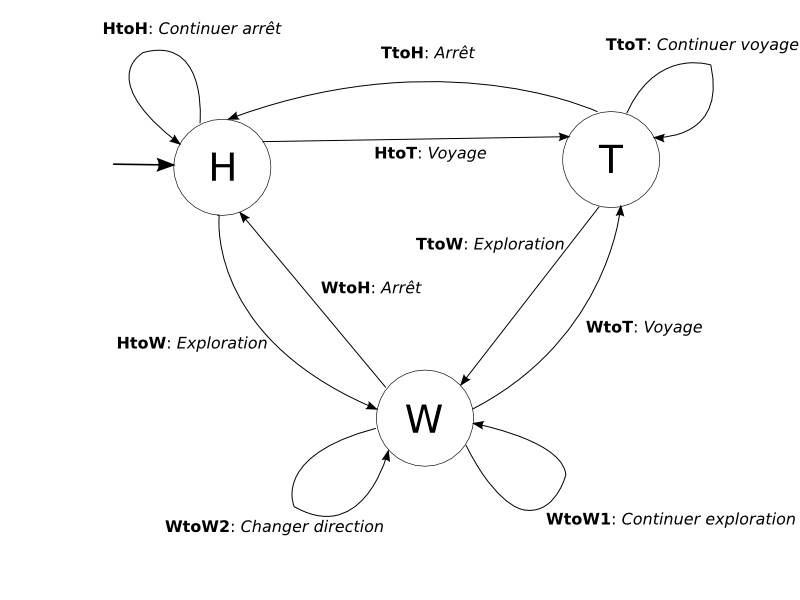
\includegraphics[scale=0.35]{images/automate.png} 
    \caption{\textit{\small Automate décrivant les mouvements d'un
        avatar. \textbf{En gras}: le nom de la transition, en \textit{italique} sa sémantique}}
    \label{fig:automate}
  \end{center}
\end{figure}
\par Nous pouvons trouver des fonctions pour faire des traitements sur les transitions, pour savoir si l'on est dans un \textit{Hotspot}, pour regarder autour, pour savoir si l'on est loin de la destination, etc. 
\par La fonction \textit{nextStep} va être étudier un petit peu plus profondément. La fonction de décompose en fonction de l'état dans lequel nous nous trouvons. Dans chaque état, des calculs (avec les probabilités définies dans le fichier de configuration) sont fait pour savoir si l'on reste dans l'état actuel ou si l'on va dans un autre état (voir figure~\ref{fig:automate}).

\section{Le fichier: \textit{GiftWrapping}}


\newpage
\bibliographystyle{plain}
\bibliography{Biblio}


 

\end{document}

